\documentclass[answers]{exam}

\usepackage{kpfonts}
\usepackage{amsmath}
\usepackage{mathabx}
\usepackage{mathtools}
\usepackage{tikz}
\usepackage{dirtytalk}
\usepackage{epigraph}


\setlength{\epigraphwidth}{0.6\textwidth}

\title{Proofs in Three Bits or Less}
\author{Math Circle}

\begin{document}

\maketitle

We started Math Circle today by introducing computational complexity, focusing on how `complex' certain \emph{algorithms} are. To do this, we introduced the idea of a \emph{worst case analysis of the problem}; with any algorithm, we associate a function $T$, such that for each positive integer $n$, $T(n)$ gives the most number of steps an algorithm will take to compute an answer to a problem of `size $n$' (the size depends on the problem; in the case of a list of numbers, we might take $n$ to be the \emph{size} of the list). To make our problems more insensitive to ambiguity, and to focus on the important parts of the function, we introduced the \emph{computational complexity classes} $\Theta(1)$, $\Theta(n)$, $\Theta(n^2)$, etc, which give the `highest order of growth' of the function. In these first set of questions, you'll find algorithms to solve problems, and investigate the complexity classes of the algorithms you create.

%Fancy algorithms are slow when N is small, and N is usually small.
%Rob Pike

\section{Complexity Theory}

\epigraph{The world is a thing of utter inordinate complexity and richness and strangeness that is absolutely awesome.}{\textit{Douglas Adams}}

%The art of simplicity is a puzzle of complexity. (Douglas Horton)

\begin{questions}

\question In the beginning of the talk, we discussed two basic algorithms for determining whether a list of numbers (for simplicity, two digit numbers) contained a particular value. Assume that checking whether two digits numbers are equal takes two basic computational steps. Can you think of a list of numbers where the first algorithm is able to finish \emph{faster} than the second algorithm (it finishes it's computation in fewer steps), and another list of numbers where the second algorithm is able to finish \emph{faster} than the first algorithm?

\question Again consider the problem of determining whether a list of numbers contained a particular value. The two algorithms above have complexity $\Theta(n)$, where $n$ is the size of the list. Thus if you were given a list of $1000$ numbers, in the worst case it would take approximately $1000$ to $2000$ steps to determine whether this list contained a particular number. Now assume that instead of an arbitrary list, we are given a \emph{sorted} list of numbers. Can you find a faster algorithm to determine if a particular number is in the list? The fastest algorithm to determine this should take roughly $10$ to $20$ steps to finish in the worst case. If you apply your list to a sorted list of $n$ numbers, what is the worst case number of steps your algorithm could take to conclude. Equivalently, what is the complexity class of your algorithm? 

\question The \emph{Fibonacci} numbers are the infinite sequence
%
\[ 1,1,2,3,5,8,13,21,34,55,89,\dots, \]
%
where each number in the sequence is obtained by adding the previous two numbers in the sequence. Find an algorithm to compute the $n$th Fibonacci number. What is the complexity class of this algorithm? Can you find a faster algorithm?

\question The next problem discussed a problem about \emph{graphs}. A graph is a collection of \emph{vertices}, together with \emph{edges} connecting them. Two vertices are \emph{adjacent} if there is an edge connecting them.

\begin{center}
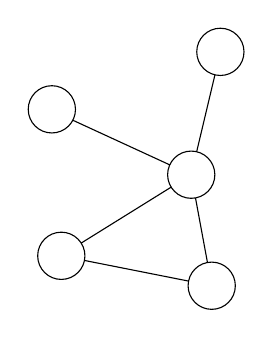
\begin{tikzpicture}[scale=0.1]
\draw [black] (29,-20.5) circle (3);
\draw [black] (50.4,-13.2) circle (3);
\draw [black] (46.7,-28.8) circle (3);
\draw [black] (30.2,-39.1) circle (3);
\draw [black] (49.3,-42.9) circle (3);
\draw [black] (33.14,-39.69) -- (46.36,-42.31);
\draw [black] (47.24,-31.75) -- (48.76,-39.95);
\draw [black] (32.7,-37.5) -- (44.15,-30.38);
\draw [black] (49.71,-16.12) -- (47.39,-25.88);
\draw [black] (31.7,-21.9) -- (43.97,-27.55);
\end{tikzpicture}
\end{center}

Graphs are super useful in many areas of mathematics, and many applications of mathematics to problems in the real world. You could model the streets of Madison as a graph, where each vertex is an intersection of roads, and two intersections are connected if there is a road leading directly from one intersection to the other. You could also use graphs to model relationships between people. Each vertex could correspond to a person, and two vertices could be connected if they correspond to people that are friends. Or you could form a family tree, where two edges connect parents to their children. Mathematical problems about graphs would then tell you about the streets of Madison, or the relationships between people.

A \emph{colouring} of a graph associates with each vertex of the graph a particular colour, such that no adjacent vertices share the same colour. If we consider a graph where each vertex corresponds to a country in the world, and two countries are adjacent if they share a border with one another, then a colouring would be precisely a colouring you could use on a world map (it would be difficult to distinguish between two countries on a map bordering one another if they shared the same colour).

If the colouring only uses two colours (say, red and blue) then we say that the colouring is a \emph{two colouring}. Can you find an algorithm to determine whether a graph is two colourable? What is it's complexity class? Can you find an algorithm to determine whether a graph is three colorable?

\question (Bonus Question) Given a graph, and two vertices in that graph, can you find an algorithm that finds the \emph{shortest number of edges} that connect the two vertices? What is it's complexity class?

\vspace{3em}

\question (Bonus Question) We say a problem is `in $\mathbf{P}$' if there exists an algorithm to compute the answer to a problem in time $\Theta(n^k)$ for some $k \geq 0$ (finding an element of a list is in $\mathbf{P}$ because we have an algorithm that takes $\Theta(n)$ time to compute an answer). Almost all of the problems in this section are `in $\mathbf{P}$'. Which problem were you not able to verify was in $\mathbf{P}$.

\end{questions}

\section{Interactive Proofs}

\epigraph{What is intuitively required from a theorem-proving procedure?
First, that it is possible to “prove” a true theorem. Second, that
it is impossible to “prove” a false theorem. Third, that communicating the proof should be efficient, in the following sense. It
does not matter how long must the prover compute during the
proving process, but it is essential that the computation required
from the verifier is easy.}{\textit{Goldwasser, Micali, Rackoff}}

In the last section, we considered algorithms which took in problems, and found solutions to those problems. In this section, we consider algorithms that \emph{take in a solution as input}, and determine if this solution is a correct solution. We call this \emph{proof verification}, since a solution is \emph{proof that something is true}, and we are checking whether this proof is legitimate (we only care about checking proofs that something is true, since checking proofs that something is false can often be a very different problem). One way we can think of this is checking these solutions for mistakes. More cynically, we can think of the solver of the problem as perhaps maliciously lying about their knowledge. This is especially important nowadays, when computers verify the identities of one another by sending solutions to very difficult math problems, that could only be solved by a particular individual with possession of some help solving the problem (a password). Either with mistakes or with maliciousness, we should be thorough in how we check our solutions. We need our proof verification algorithms to be both:
%
\begin{itemize}
    \item \emph{Perfectly Complete}: If a solution is correct, we will verify the solution correctly.

    \item \emph{Perfectly Sound}: If a solution is incorrect, we will throw out the solution.
\end{itemize}
%
Let's consider some examples of proof verification.

\begin{questions}

	\question In the last set of problems, we considered the \emph{three coloring problem}, which takes $\Theta(3^n)$ steps to find a coloring if it exists, or to show no coloring exists. Can you find an algorithm that takes in as input a three coloring for the problem, and then \emph{checks} whether a three coloring is valid. What is it's complexity? 

	\question Consider an algorithm that takes in an input a proof that a particular number is in a list, and checks whether this proof is valid? What is it's complexity? What would a proof that a number is \emph{not} in a list look like?

	\question We say two graphs are \emph{equivalent} if, after rearranging the vertices of the graph, you have the same graph. For instance, the following two graphs are equivalent:
	%
	\begin{center}
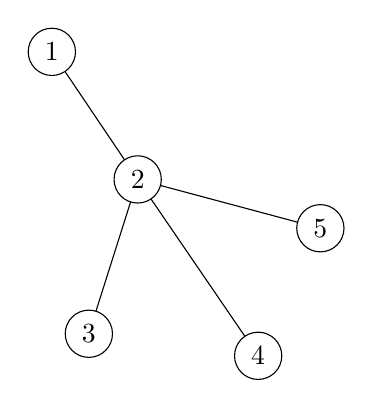
\begin{tikzpicture}[scale=0.1]
\tikzstyle{every node}+=[inner sep=0pt]
\draw [black] (33.1,-22.5) circle (3);
\draw (33.1,-22.5) node {$2$};
\draw [black] (56.3,-28.7) circle (3);
\draw (56.3,-28.7) node {$5$};
\draw [black] (26.9,-42.1) circle (3);
\draw (26.9,-42.1) node {$3$};
\draw [black] (48.4,-44.9) circle (3);
\draw (48.4,-44.9) node {$4$};
\draw [black] (22.2,-6.3) circle (3);
\draw (22.2,-6.3) node {$1$};
\draw [black] (27.8,-39.24) -- (32.2,-25.36);
\draw [black] (46.71,-42.42) -- (34.79,-24.98);
\draw [black] (53.4,-27.93) -- (36,-23.27);
\draw [black] (31.43,-20.01) -- (23.87,-8.79);
\end{tikzpicture}\quad\quad\quad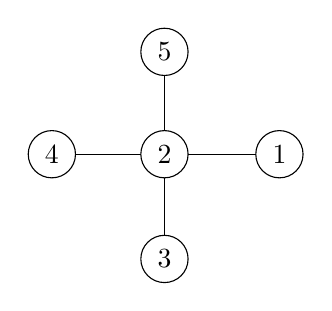
\begin{tikzpicture}[scale=0.1]
\tikzstyle{every node}+=[inner sep=0pt]
\draw [black] (45.2,-29.9) circle (3);
\draw (45.2,-29.9) node {$2$};
\draw [black] (45.2,-16.9) circle (3);
\draw (45.2,-16.9) node {$5$};
\draw [black] (45.2,-43.2) circle (3);
\draw (45.2,-43.2) node {$3$};
\draw [black] (30.9,-29.9) circle (3);
\draw (30.9,-29.9) node {$4$};
\draw [black] (59.8,-29.9) circle (3);
\draw (59.8,-29.9) node {$1$};
\draw [black] (45.2,-40.2) -- (45.2,-32.9);
\draw [black] (33.9,-29.9) -- (42.2,-29.9);
\draw [black] (45.2,-19.9) -- (45.2,-26.9);
\draw [black] (48.2,-29.9) -- (56.8,-29.9);
\end{tikzpicture}
\end{center}
%
Given two graphs, what would a `proof' that two graphs are equivalent look like? What would a `proof' that two graph are \emph{not} equivalent look like?

\end{questions}

A problem is `in $\mathbf{NP}$' if there exists a way of checking solutions to a problem that have time complexity $\Theta(n^k)$ for some $k \geq 0$. In question 6 of the last section, we consider the class of problems `in $\mathbf{P}$'. Intuitively, it is easier to `mark an exam' then to `take an exam'. We even have phrases in english, such as `it's easier to be a critic than a creator'. Thus one might conjecture that the class of problems $\mathbf{NP}$ contains more difficult problems than the class $\mathbf{P}$. We might write this as $\mathbf{P} \neq \mathbf{NP}$. But despite being posed over 50 years ago, it is still completely unknown whether $\mathbf{P} = \mathbf{NP}$, or whether $\mathbf{P} \neq \mathbf{NP}$. At the turn of the millenium, a one million US dollar prize was offered to anyone who might be able to resolve this problem. But we are still nowhere close to resolving the problem. It's often the most fundamental problems in mathematics that remain unsolved for so long.

\section{Probabilistically Checkable Interactive Proofs}

\epigraph{Suppose a mathematician circulates a proof of an important result, say Riemann Hypothesis, fitting several thousand pages. To verify it would take you and
your doubting colleagues several years. Can you do it faster? Yes, according to the
PCP Theorems. He can rewrite his proof so you can verify it by probabilistically
selecting 3 bits to examine in it.}{\textit{Sanjeev Arora}}

Suppose we don't want to be as thorough in our marking. If we only want to spot \emph{most} mistakes, is the complexity of our problem reduced? Let's be precise about how we do this. It turns out that, amazingly, you can reduce the complexity of the problem \emph{immensely}, such that every problem `in $\mathbf{NP}$' can be checked in \emph{at most 3 steps}. In three steps, we can only really ask three `yes or no' questions about the solution to the problem. So we can think of these proof verifiers as being almost like players of the game `20 questions', or `Guess Who'. We must extract the maximal amount of information about a solutions to a problem in as minimal a number of questions as possible.

Let's be precise about the amount of error we are allowed in the problem. We consider a \emph{random} algorithm, that chooses a set of questions to ask in a random manner, such that we have:
%
\begin{itemize}
	\item \emph{Imperfect Completeness}: If a statement is true, then we will accept the solution with probability $\geq 1/2$

	\item \emph{Imperfect Soundness}: If a statement is false, then we will reject the solution with probability $\leq 1/2$.
\end{itemize}
%
The particular probability bound $1/2$ doesn't really matter here, since iterating the algorithm repeatedly will decrease the amount of error in the problem; if we run the algorithm $m$ times in a row, then we will accept true solutions with probability $\geq 1 - 1/2^m$, and reject false solutions with probability $\leq 1/2^m$. We call such an algorithm a \emph{probabilistically checkable proof}.

Here's an example of a probabilistically checkable proof, which examines a solution to the problem of when two graphs are \emph{not equivalent}, as in Question 3. After puzzling aruond with this problem, you might have seen that a proof that two graphs are not equivalent with \emph{perfect completeness} and \emph{perfect soundness} (no errors) can be very very long. But we can check whether two graphs $G$ and $H$ are not equivalent with \emph{a single question}. The idea is simple. We flip a coin, and pick one of the graphs $G$ and $H$ depending on the outcome of the coin toss. Then we shuffle all of the vertices and edges of the graph, thus hiding which graph we originally chose. We ask the prover of the non-equivalence statement to identify which of the graphs we began with as part of the solution they are submitting to us. If the prover is correctly able to identify the original graph, we accept their solution. If the prover incorrectly identifies a graph, we reject their solution.

This interactive proof has \emph{perfect completeness}; if the prover gives a valid solution to the problem, we will always accept their solution. It also has \emph{imperfect soundness}: Suppose that a person \emph{claimed} to have shown the two graphs were not equivalent, but that the graphs were in actuality equivalent to one another. In the interactive proof above, since the two graphs are equivalent, the prover will have no way to tell which of the two graphs we began with, since the problem we gave them to solve is equally likely to have come from either of the two equivalent graphs. Thus the prover is bound to fail with probability at least $1/2$.

Let us try and consider a probabilistically checkable proof that two graphs are three colorable. We might ask the prover to submit a three coloring. We then select two adjacent vertices at random, and check whether they are the same color. If they are, we reject the solution. If they aren't we accept the solution. Since we only check the colors of \emph{two of the vertices}, this probabilistically checkable proof only asks two questions. This algorithm has perfect completeness, since a correct solution will never be rejected. If the graph is not three colorable, there will be at least one pair of adjacent vertices which are colored the same, so our algorithm will reject this solution with probability $\geq 1/E$, where $E$ is the number of edges in the graph. This doesn't quite give imperfect soundness, since $1/E$ can be much smaller than $1/2$, unless we had some guarantee that every coloring of the graph would fail on at least half of the adjacent edges. We call such a graph an \emph{expander}. Thus we have a probabilistically checkable proof, at least for the class of expander graphs.

\newpage

\begin{center}
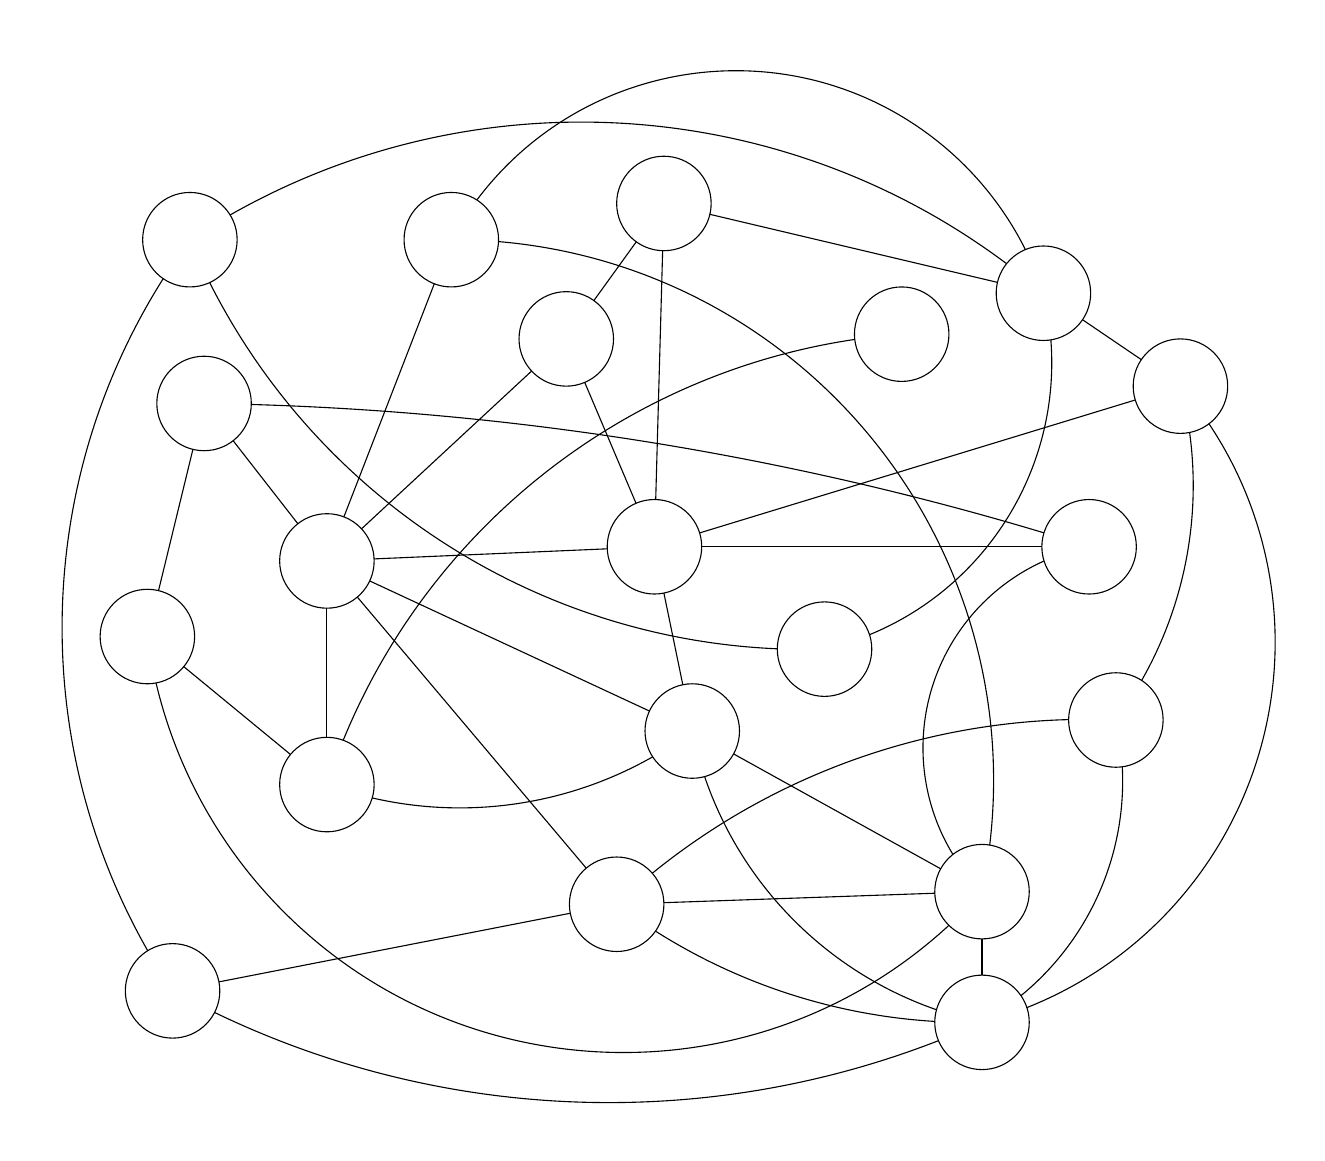
\begin{tikzpicture}[scale=0.2]
\tikzstyle{every node}+=[inner sep=0pt]
\draw [black] (27,-5.9) circle (3);
\draw [black] (40.5,-3.6) circle (3);
\draw [black] (11.3,-16.3) circle (3);
\draw [black] (39.9,-25.4) circle (3);
\draw [black] (19.1,-26.3) circle (3);
\draw [black] (64.6,-9.3) circle (3);
\draw [black] (60.7,-47.3) circle (3);
\draw [black] (37.5,-48.1) circle (3);
\draw [black] (19.1,-40.5) circle (3);
\draw [black] (34.3,-12.2) circle (3);
\draw [black] (42.3,-37.1) circle (3);
\draw [black] (67.5,-25.4) circle (3);
\draw [black] (7.7,-31.1) circle (3);
\draw [black] (50.7,-31.9) circle (3);
\draw [black] (10.4,-5.9) circle (3);
\draw [black] (9.3,-53.6) circle (3);
\draw [black] (69.2,-36.4) circle (3);
\draw [black] (55.6,-11.9) circle (3);
\draw [black] (73.3,-15.2) circle (3);
\draw [black] (60.7,-55.6) circle (3);
\draw [black] (8.41,-28.18) -- (10.59,-19.22);
\draw [black] (10.01,-33.01) -- (16.79,-38.59);
\draw [black] (19.1,-29.3) -- (19.1,-37.5);
\draw [black] (21.03,-28.59) -- (35.57,-45.81);
\draw [black] (17.25,-23.93) -- (13.15,-18.67);
\draw [black] (20.18,-23.5) -- (25.92,-8.7);
\draw [black] (21.3,-24.26) -- (32.1,-14.24);
\draw [black] (21.82,-27.57) -- (39.58,-35.83);
\draw [black] (41.7,-34.16) -- (40.5,-28.34);
\draw [black] (38.73,-22.64) -- (35.47,-14.96);
\draw [black] (44.92,-38.55) -- (58.08,-45.85);
\draw [black] (57.7,-47.4) -- (40.5,-48);
\draw [black] (42.9,-25.4) -- (64.5,-25.4);
\draw [black] (36.05,-9.77) -- (38.75,-6.03);
\draw [black] (43.42,-4.29) -- (61.68,-8.61);
\draw [black] (40.42,-6.6) -- (39.98,-22.4);
\draw [black] (22.1,-26.17) -- (36.9,-25.53);
\draw [black] (58.598,-49.439) arc (-47.32231:-166.67033:30.498);
\draw [black] (28.622,-3.379) arc (143.06116:26.60494:20.571);
\draw [black] (39.789,-38.738) arc (-60.35081:-102.9743:24.768);
\draw [black] (29.997,-6.021) arc (85.17851:-6.88667:34.325);
\draw [black] (12.24,-53.03) -- (34.56,-48.67);
\draw [black] (7.721,-51.05) arc (-150.3158:-212.3263:41.434);
\draw [black] (14.299,-16.364) arc (88.3288:73.276:194.643);
\draw [black] (47.701,-31.879) arc (-92.42597:-153.23111:42.381);
\draw [black] (12.956,-4.33) arc (119.64479:53.17622:45.069);
\draw [black] (65.072,-12.259) arc (4.46642:-67.65313:18.676);
\draw [black] (70.43,-16.08) -- (42.77,-24.52);
\draw [black] (70.82,-13.52) -- (67.08,-10.98);
\draw [black] (73.883,-18.141) arc (7.7692:-29.66051:24.994);
\draw [black] (39.763,-46.131) arc (129.05701:91.4597:43.726);
\draw [black] (20.136,-37.685) arc (157.73427:98.42751:41.705);
\draw [black] (58.856,-44.942) arc (-148.58818:-245.91119:13);
\draw [black] (60.7,-52.6) -- (60.7,-50.3);
\draw [black] (69.608,-39.368) arc (2.9539:-50.71265:17.611);
\draw [black] (57.701,-55.54) arc (-93.45165:-122.37788:37.314);
\draw [black] (57.811,-54.799) arc (-109.11231:-161.19824:23.781);
\draw [black] (57.935,-56.762) arc (-68.70225:-115.75432:57.623);
\draw [black] (75.112,-17.589) arc (33.73167:-68.37511:24.968);
\end{tikzpicture}
\end{center}

\end{document}